\documentclass[man]{apa2}
\usepackage{pslatex}
\usepackage{amssymb}
\usepackage{graphicx}
\usepackage{color}
\usepackage{covington}
\usepackage[usenames,dvipsnames]{xcolor}
\usepackage{booktabs}
\usepackage{setspace}
\usepackage{textgreek}

\title{The trouble with quantifiers: Children's difficulty with scalar terms extends beyond the realm of implicatures}

\threeauthors{Alexandra C. Horowtiz}{Rose M. Schneider}{Michael C. Frank}
\threeaffiliations{Department of Psychology, Stanford University}{Department of Psychology, Stanford University}{Department of Psychology, Stanford University}

\abstract{Both production and comprehension of language often require speakers and listeners to make pragmatic inferences beyond the literal sense of the utterance, particularly in the case of pragmatic implicatures. Adult listeners quickly and easily infer from the utterance ``\textit{Some} of these cookies are oatmeal raisin'' that the other cookies might be chocolate chip. On the other hand, children have more difficulty with this statement; previous research has suggested that children succeed in making implicatures in some cases but not others. However, children's performance varies tremendously across studies and tasks, limiting the number of possible direct comparisons between datasets. To address this issue, we designed a novel experimental paradigm, which both minimized task demands for participants, and enabled comparisons across different tasks. In Experiment 1, we used this paradigm to explore children's ability to compute both ad-hoc (contextual) and scalar (quantifier) implicatures, and found that while older 4-year-olds performed at ceiling for ad-hoc descriptions, they still performed poorly with scalar descriptions. In Experiment 2, we attempted to isolate children's sources of difficulty with these terms by including only scalar trials, and found that while performance increased, it was still low. Particularly, we observed a positive correlation between performance with the scalar terms ``some'' and ``none''. In Experiment 3, we explored possible sources of developmental difficulty in this task, combining our paradigm with tests of inhibitory control and quantifier knowledge. After controlling for age, we found that inhibitory control did not predict the ability to make scalar implicatures, but that children who had difficulty with ``some'' and ``none'' in an implicature task also had issues with these scalar terms in the quantifier knowledge task. Taken together, our results provide easily comparable developmental data on the development of pragmatic implicatures, and suggest that sources of difficulty over this development are not confined to making implicatures, but may be affected by quantifier knowledge and other pragmatic and processing demands.
~\\

Keywords: pragmatics, development}

\shorttitle{The trouble with quantifiers}
\rightheader{The trouble with quantifiers}

\acknowledgements{ We gratefully acknowledge. 

~\\

\noindent Address all correspondence to Rose M. Schneider, Stanford University, Department of Psychology, Jordan Hall, 450 Serra Mall (Bldg. 420), Stanford, CA, 94305. Phone: 650-721-9270. E-mail: \texttt{rschneid@stanford.edu}.}

\begin{document}

\maketitle               

\section{Introduction}
Why are implicatures important? 

What are the developmental differences?

Why is this interesting?

What are some of the sources of difficulty with children understanding implicatures? 

Stiller et al. 

Previous studies examine implicatures using differing methods, and the results are difficult to compare

Introduce new paradigm for adhoc and scalar implicature research 


\subsection{Previous work}

In study 1,  one paradigm provides reliable and consistent measurement of implicature performance in children 3-5; however, children succeed with ad hocs, but have difficulty with scalar items; given that children were successful in computing ad hoc implicatures with this paradigm, could the poor performance in these scalar trials be due to the fact that the trials were intermixed with the adhoc trials?

In study 2, we examined this possibility by only testing scalar items, and found that while this increased performance for older children, children were still having difficulty with this task, particularly with the ``some'' and ``none'' trials

Children who had problems with ``some'' were also more likely to have issues with ``none'' 

There are several reasons we might have seen the results that we did

Children may need to know both ends of the quantifier scale in order to be able to make an implicature

There might be problems with inhibition; children in these trials might listening through the quantifier and answering purely based on the target noun; this is supported by the fact that children reliably choose ?all? for ``some'' and ``none'' trials

Do children not know what these quantifiers mean?

In study three, we explored these alternatives by running children on both the SI task, an inhibitory control task (DCCS) as well as the Give-Quantifier task, a productive measure of quantifier knowledge

Interestingly, we found that the patterns of performance persist in SI as in Horowitz and Frank, and that DCCS was not predictive of performance in either SI or GQ when controlled for age

However, we found correlations between the Give-Quantifier task with ?some? and ?none? trials (except for GQ none and SI some, I think) when controlling for age; this seems to indicate that difficulties with these scalar terms exist outside of the implicature realm

Children just seem to have a trouble with quantifiers


\section{Experiment 1: Ad hoc and scalar implicature computation in children}

Given the difficulty in equating results on children's computation of implicatures across different methods and paradigms, we created a single task that could be adapted to investigate both ad hoc and scalar items in one task. This task involved one set of stimuli presented in the same order to all participants; however, the particular items queried were counterbalanced across participants. Thus, with one set of stimuli we created a novel paradigm wherein we could directly compare children's performance on both ad hoc and scalar implicatures in a single experimental session. In Experiment 1, we included questions about ad hoc and scalar implicatures within one session, and found that this paradigm was appropriate for ad hoc items, but children still experienced difficulty computing scalar items.

% In Experiment 2, we included only scalar items in the task, and found that participants were moderately more successful at making implicatures when these trials were presented in isolation. In Experiment 3, we explored two alternatives potentially driving children's difficulties in this task.  

\subsection{Methods}

\subsubsection{Participants} A planned sample of 48 children was recruited from Bing Nursery School at Stanford University. These children were drawn from two age groups: twenty-four 4.0 -- 4.5-year-olds (M = 4;2, median = 4.19, SD = 0.14) and 24 4.5 -- 5.0-year-olds (M = 4.74, median = 4.73, SD = .16). Two children were excluded from the final sample for not completing the task, and one additional child was excluded due to experimenter error. The final sample was comprised of (XX males and XX females) with English as their primary language. Across all experiments, no child completed more than one session of the task. 

\begin{figure} 
 \begin{center} 
  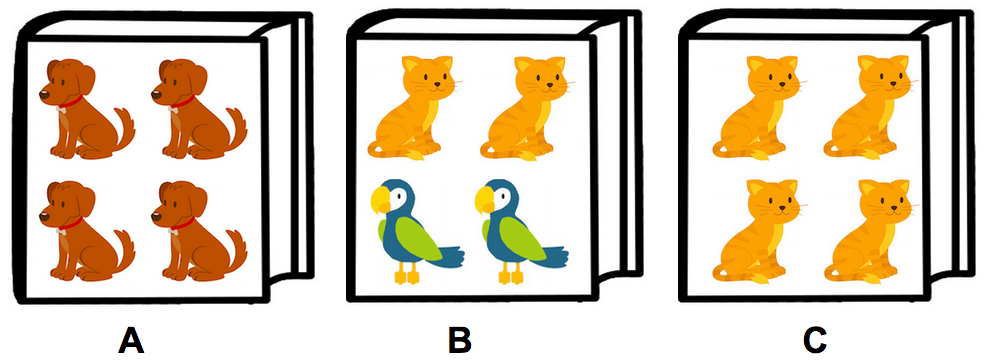
\includegraphics[height=2in]{figures/implicatures_demo_letters.png} 
  \caption{\label{fig:demo} Example trial stimuli used in all experiments. Children received a clue from the experimenter about which book she had in mind and responded based solely on the clue; this was either an ad hoc or a scalar description of a book with either an unambiguous or implicature target.} 
 \end{center} 
\end{figure}	 

\subsubsection{Stimuli}
Stimuli for all experiments were created to be appropriate for questions about both ad hoc and scalar implicatures, allowing the experimenter to use one set of stimuli for both kinds of items in one experimental session. The experimental stimuli consisted of a set of printed pictures of three book covers with four familiar items on each cover. In each trial, one book cover contained four items of the same kind (e.g., four cats), another book cover contained four items of another kind (e.g., dogs), and the final cover contained two items of a new set and two items repeated from one of the other book covers (e.g., two birds and two cats). An example of the stimuli can be seen in Figure \ref{fig:demo}. Experiment 1 consisted of 18 test trials preceded by one test trial, with three book covers containing only one familiar item. All items on the book covers were familiar to children, and were able to be identified. All participants saw the same book covers in the same order. 


\subsubsection{Procedure}
Participants were tested in individual sessions in a quiet room at their nursery school. The experimenter introduced the study as a guessing game, and explained that the child would receive a hint about which book cover the experimenter had in mind. In the instructions for the task, the experimenter emphasized that the child would only receive one clue about what book the experimenter was describing, and they had to use that clue to make their decision. All participants saw the same book covers in the same order; however, (three?) scripts with both ad-hoc and scalar trials were counterbalanced across participants. A breakdown of trial types and sample scripts can be seen in (Table 1). 

Prior to the test trials, children were familiarized to the task with a practice trial. The practice trial consisted of three book covers, each displaying a single unique and familiar item. After children had successfully completed the practice, children saw 18 test trials with stimuli of books containing sets of familiar items. At the start of every trial, the experiment would provide the child with either an ad-hoc or scalar description of one of the books and instruct the child to point to the book she was describing. If the child pointed to more than one book, or the response was otherwise ambiguous, the experimenter emphasized again that she was talking about just one book, and that they should choose the single book she was describing. 

In ad-hoc trials (eight total), the experimenter's descriptions of the target book used names of the pictured objects, providing contextual support for the target. Ad-hoc control trials referred to an unambiguous target (e.g., ``On the cover of my book, there are dogs'' in Figure \ref{fig:demo}). while implicature trials required the child to reason about the speaker's meaning given the ambiguous utterance (e.g., ``On the cover of my book, there are cats'', which could refer to either the book containing only cats or the book containing cats and birds). In these critical trials, children had to understand that the speaker could potentially be talking about either the book with four or two of the named object, but that by opting to describe only one kind of object she was referring to the cover with four of the same object; otherwise, she would have mentioned both kinds of objects, or the ones unique to that cover (i.e., birds). 

In scalar trials (ten total), the experimenter described the target book with quantifiers. For scalar items, control trials referred to unambiguous targets with the quantifiers ``all'' and ``none'' (e.g., ``On the cover of my book, \textit{all/none} of the pictures are cats'') or an unambiguous referent of ``some'' (e.g., ``On the cover of my book, \textit{some} of the pictures are birds''). On critical scalar implicature trials, the experimenter used the weak quantifier ``some'' to reference the item pictured across two book covers (e.g., ``On the cover of my book, \textit{some} of the pictures are cats''). These trials required the child to reason that because the speaker used the weak quantifier ``some'', some must be referring to the book picturing only two of the named target, or else she would have used the strong quantifier ``all''. 

All participants saw image sets in the same order; however, these image sets were counterbalanced for target location and book triad position. Description condition and trial-type were further randomized across participants, and were spaced to avoid immediate repeat trial types. Children did not receive feedback after the test trial.

\subsection{Results}


\begin{figure} 
 \begin{center} 
  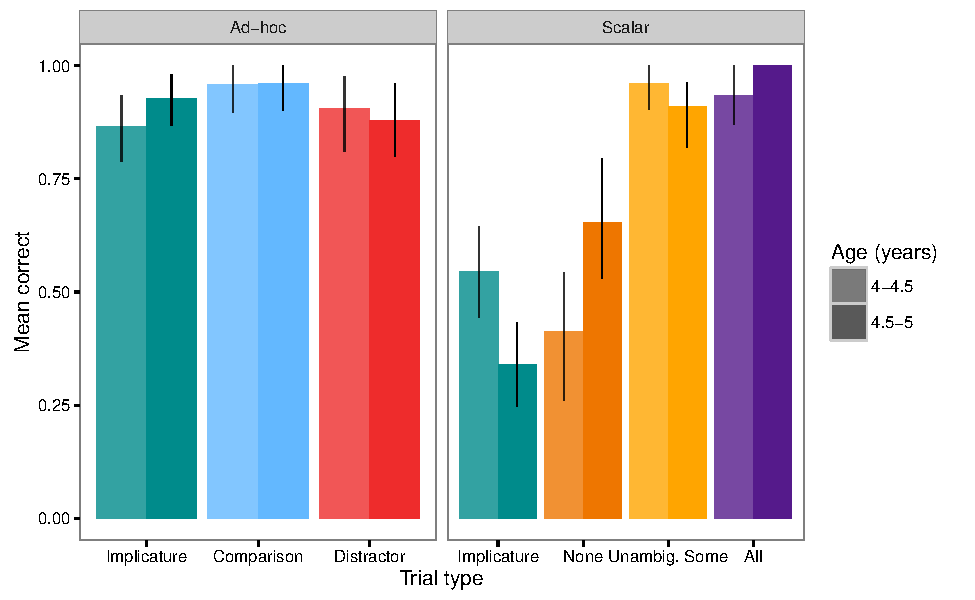
\includegraphics[height=2in]{figures/exp1_performance.pdf} 
  \caption{\label{fig:exp1_perf} Proportion of correct responses by each age group across all trial types and split by implicature type. Error bars show standard error of the mean. Children performed almost at ceiling in ad-hoc implicature conditions, but struggled in scalar trials, particularly in the ``some'' and ``none'' trials.} 
 \end{center} 
\end{figure}

Children's performance on all trial types can be seen in Figure \ref{fig:exp1_perf}. Across all trials, children's performance was coded as correct if they selected the image consistent with either the ad-hoc or scalar description. Children were at ceiling making ad-hoc implicatures, which is consistent with previous research suggesting that children are able to succeed in making such implicatures when they have access to the relevant lexical alternatives \cite{Stiller2014}. Children's performance across ad-hoc trials provides strong evidence that our novel paradigm is an appropriate measure for such items.

In contrast to their success in making ad-hoc implicatures, children struggled in scalar trials. Although they succeeded in ``all'' and ``unambiguous some'' trials, children performed near chance on ``some'' and ``none'' trials. 

%This is lifted directly from Ali's cogsci paper
We ran a logistic mixed effect model, predicting a correct response as an interaction of age, condition (ad-hoc or scalar) and trial type (implicature or control), with random effects of participant and trial type. We found that performance was slightly lower for scalar trials than ad-hoc trials ($\beta$= --8.02, \textit{p} = .09), and that there was a significant interaction between condition and trial type, such that performance was significantly worse on scalar implicature trials ($\beta$= 16.45, \textit{p} \textless  .02). We also found a significant 3-way interaction between condition, trial type, and age, such that performance on scalar implicature trials decreased with age ($\beta$ = --4.16, \textit{p} \textless  .01). There were no significant effects of adding trial order (trials in the first half vs. second half of the experiment), indicating that performance did not change throughout the course of the experiment. 

Interestingly we found that when children's performance in scalar trials varied consistently. To examine their patterns of responses more closely, we ran Hartigan's dip test and found significant bimodal distributions for both \textit{some} (\textit{D} = .15, \textit{p} \textless  .0001) and \textit{none} (\textit{D} = .20, \textit{p} \textless  .0001). This suggests children did not respond at chance in scalar trials, but either consistently correctly or incorrectly. Additionally, children's success on \textit{some} and \textit{none} trials was highly correlated (\textit{r} = .47, \textit{p} \textless  .001), such that children who performed better on some trials also tended to perform better on none trials.  Performance on \textit{none} and \textit{all} trials (\textit{r} = .11, \textit{p} = .45) and \textit{some} and \textit{all} trials (\textit{r} = .01, \textit{p} = .95) was not correlated. 

\subsection{Discussion}

The results of Experiment 1 indicated that while children were easily able to make ad-hoc implicatures in our task, they had difficulty making scalar implicatures. This pattern of performance was puzzling, given both our efforts to reduce task demands and children's striking success in ad-hoc trials. In spite of having access to both visual alternatives (the three selection choices) within each trial and lexical alternatives across all trials, children were still at chance in making scalar implicatures in our task. 

Even more intriguing was the unexpected developmental change we observed on \textit{none} trials. We chose to include ``none'' as an unambiguous control quantifier, but found that children performed at chance for this scalar term as well. These results are supported by previous work suggesting that even older preschoolers struggle with negation occurring in arbitrary contexts \cite{nordmeyer2014}. Given children's difficulty with ``none'' and the strong positive correlation between \textit{some} and \textit{none} trials, it is possible that making implicatures necessitates some familiarity with both ends of the quantifier scale (\textit{none -- some -- all}).

In addition to understanding the extremes of the quantifier scale, two other possibilities -- namely, lack of quantifier knowledge, and inhibitory control -- may also account for children's decreased performance on scalar items. However, we also wondered if these results were the effect of including both ad-hoc and scalar quantifier descriptions within one experimental session. It is possible that children's success on ad-hoc trials may have to a misinterpretation of a scalar description (e.g., ``On the cover of my book, some of the pictures are cats'') to an ad-hoc one (``On the cover of my book, there are cats''). There is some evidence that children will sometimes rely exclusively on one strategy to solve problems, even if another strategy is more appropriate (citing Ann's work from the summer, maybe?). 

To further explore the possibility that children's performance on scalar trials might have been influenced by ad-hoc trials, we removed all ad-hoc trials from our task, and ran a scalar-only version of the the study.

\section{Experiment 2: Isolating scalar implicatures}
In Experiment 2, we pursued the possibility that children might be failing in making scalar implicatures as a result of competing ad-hoc descriptors contained in the same experimental session. Additionally, we expanded our sample age-range to 3--5 years in order to more fully explore the developmental trajectory of scalar implicature comprehension. 

\subsection{Methods}
\subsubsection{Participants} 

We recruited a new sample of 50 participants from Bing Nursery School at Stanford University: 12 3.0--3.5-year-olds (M=3;4), 12 3.5--4.0-year-olds (M=3;8), 14 4.0--4.5-year-olds (M=4;3), and 12 4.5--5.0-year-olds (M=4;8). One additional child was excluded for stopping the task early.

\subsubsection{Stimuli}
Stimuli were identical to Experiment 1. The only changes made in experimental protocol were to the scripts; ad-hoc trials were dropped, and all 18 test trials were converted to scalar descriptions (Table XX). In Experiment 2, the 18 test trials consisted of six control \textit{all} trials (e.g., ``On the cover of my book, \textit{all} of the pictures are cats''), six \textit{none} trials (e.g., ``...\textit{none} of the pictures are cats''), and six scalar implicature trials (``...\textit{some} of the pictures are cats''). We removed the unambiguous references to \textit{some} to more effectively counterbalance trials; in scalar implicature trials, the quantifier always referenced the item pictured across two book covers (e.g., in Figure \ref{fig:demo}, children heard references to \textit{none, some,} or \textit{all} cats). As in Experiment 1, image sets were presented in a fixed order, counterbalanced for both target location and triad order. Participants were randomly assigned to one of three scripts, with a pseudo-randomized trial order such that every book set was referred to by each quantifier type, and the same trial type never immediately repeated.

\subsubsection{Procedure}
The procedure was identical to Experiment 1. 

\subsection{Results}

\begin{figure} 
 \begin{center} 
  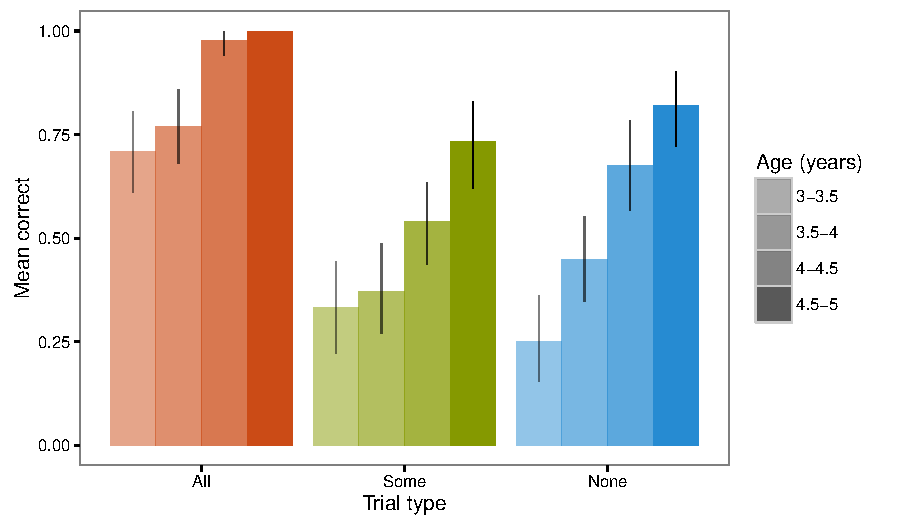
\includegraphics[height=2in]{figures/exp2_performance.pdf} 
  \caption{\label{fig:exp2_perf} Proportion of correct responses by each age group across all scalar trial types. Error bars show standard error of the mean.} 
 \end{center} 
\end{figure}

In Experiment 2, children's performance increased with age (\ref{fig:exp2_perf}. Performance was highest in \textit{all} trials, with all age groups significantly above chance. However, performance was still low in both \textit{none} and \textit{some} trials, with only the oldest age group performing above chance for \textit{none} trials (\textit{t} = 3.09, \textit{p} = .01), but only marginally above chance for \textit{some} trials (\textit{t} = 1.85, \textit{p} = .09). 

We ran a logistic mixed effects model, predicting correct responses as an interaction of age and trial type (\textit{all, some}, or \textit{none}), with random effects of trial type by participant. However, we found that the only significant effect that emerged was age, such that performance increased across trials as children got older ($\beta$ = 20, \textit{p} \textless  .001). Adding trial order (first or second half of the experiment) to the model did not interact with any of the variables, indicating the performance did not change over the course of the experiment. 

Consistent with the findings from the mixed effects model, we again found significant bimodal patterns of responses for both \textit{some} (\textit{D} = .12, \textit{p} \textless  .0001) and \textit{none} (\textit{D} = .15, \textit{p} \textless  .0001) trials. And again, these trial types were highly correlated with one another (\textit{r} = .52, \textit{p} \textless  .001). 

As a exploratory analysis, we ran another version of the mixed effects model removing the random effect of trial type. In addition to a main effect of age (\textit{t} = 1.88, \textit{p} \textless  .01), this model revealed that performance on \textit{some} trials was lower than \textit{all} trials (\textit{t} = --7.69, \textit{p} \textless  .01), and marginally reduced from \textit{none} trials (\textit{t} = 3.03, \textit{p} = .09). We also found interactions between trial type and age, such that there was a greater difference between younger children's performance on \textit{some} and \textit{all} trials (\textit{t} = 2.84, \textit{p} \textless  .001), and \textit{some} and \textit{none} trials (\textit{t} = 0.90, \textit{p} = .05). 

\subsection{Discussion}

In Experiment 1, we observed success in children's computation of ad-hoc, but not scalar implicatures. To explore whether children's performance in making scalar implicatures might be hindered by the presence of both ad-hoc and scalar items in the same session, leading them to misinterpret all descriptions as contextual. In Experiment 2, we excluded ad-hoc items, and replaced them with scalar descriptions. 

When faced with only scalar implicatures, children's performance was marginally better than in Experiment 1, with success in making a scalar implicature positively correlated with age. However, we still observed decreased performance in both the \textit{some}, as well as the unambiguous \textit{none} trials. Additionally, we again found bimodal and correlated patterns of responses in these two trials, with children making errors in implicature trials also failing on \textit{none} trials. 

The results of Experiment 2 indicated that children have difficulty with making scalar implicatures beyond dealing with competing contextual descriptors, but the cause of this developmental change is not clear. One possible explanation for this effect is that children's knowledge of the full quantifier scale is not yet adult-like in their preschool years, and that the meanings of these scalar terms may yet be established. Another possibility is that children's performance might suffer on these task from developing inhibitory control, with children not being able to overcome the impulse to select the target noun, regardless of the quantifier user. 

Based on our findings of bimodal and correlated performance and patterns of errors, we decided to explore these two alternatives in Experiment 3, and include measures of both inhibitory control and quantifier knowledge in the same session. 

%Need to make a better individual differences graph for this, also need to make a graph for what kinds of errors kids make
				
\section{Experiment 3: Inhibitory control and quantifier knowledge measures}

In an effort to explore the particular sources of difficulty for children in making scalar implicatures, in Experiment 3 we supplemented our implicature task with an inhibitory control task \cite{zelazo2006}, and a quantifier-knowledge task \cite{barner2009} in a within-subject experiment.  

\subsection{Methods}
\subsubsection{Participants} We recruited a new planned sample of 72 children from Bing Nursery School at Stanford University. Once again, we included children from 3--5 years: 21 3--3.5-year-olds (M = 3;3), 15 3.5--4-year-olds (M = 3;8), 19 4--4.5-year-olds (M=4;2), and 17 4.5--5-year-olds (M = 4;7). Twelve children were excluded from the final sample for having participated in either Experiments 1 or 2. Nine children completed one of the tasks in a different testing session. 

\subsubsection{Stimuli} The stimuli for the implicature task were identical to Experiments 1 and 2. Once again, we excluded ad-hoc items, and ran a scalar-only version of the task. Our measure of inhibitory control was the Dimensional Change Card Sort (DCCS, \cite{zelazo2006}), with materials drawn from that study. The 14 laminated sorting cards used in the study were 11cm x 7 cm, and consisted of 7 red rabbits and 7 blue boats. These cards were put into plastic sorting trays, one with a red boat, and the other with a blue rabbit. To assess quantifier knowledge, we used the Give-Quantifier task \cite{barner2009}. Stimuli for this task consisted of three different sets of plastic fruits (8 oranges, 8 bananas, and 8 strawberries) and a red plastic plate. These fruits were grouped together by kind at the start of each trial. 

\subsubsection{Procedure}
The procedure for our implicature task was identical to Experiment 2, the scalar-only version of the task. Tasks were counterbalanced across participants, and individual scripts for each task were also counterbalanced to avoid any possibility of order effects. The tasks were done in a small room apart from the main classroom in individual sessions. The experimenter asked the child before the start of every task whether she would like to play the game or return to the classroom. As the all three tasks took around 15 minutes in total, only 9 children opted to return to the classroom and finish an individual task on another day. 

We drew our protocol for DCCS directly from the original methods paper \cite{zelazo2006}. At the start of the game, the experimenter randomly chose a dimension (color or shape) that would guide the rules of the pre-switch phase of the task. The experimenter then told the child that they would be playing a game about the relevant dimension (e.g., the shape game), in which they would sort the cards by that particular dimension. Two training trials preceded the testing phase: in these training trials, the experimenter labeled the two target cards (the blue rabbit and the red boat), and then displayed a card to the participant, identified it by the relevant dimension, and then explained to the child where the card should be sorted and why. This process was repeated with another playing card before 6 pre-switch test trials. The 6 pre-switch trials each began with the experimenter holding up a card, labeling it by the target dimension, and asking the child where it should go (e.g., ``Here is a boat. Where should it go?''). The child then placed the card in the sorting tray face-down. If the child placed the card face-up, the experimenter turned it over. 

After the 6 pre-switch trials, the experimenter stopped the game briefly, and explained to the child that now they were playing a game about the other dimension (e.g., the color game), and that now they would be sorting the cards by the other dimension. The experimenter proceeded immediately into 6 post-switch trials. The first post-switch trial started with a reminder about the shifted rules of the game, then a label of the relevant dimension, and finally a question as to where it should go (e.g., ``Remember, we're playing the color game now; if it's blue it goes here, if it's red it goes here. Here is a red one; where does it go?). In the remaining test trials, the experimenter only labeled the target dimension, and asked the child where the card should go. Again, if the child did not place the card face-down, the experimenter turned it over. The pre-switch dimension was chosen randomly at the start of the task, and cards were shuffled after the two training cards. 

In running the Give-Quantifier task, we followed the methods of the original task fairly closely, with the exception of a few minor modifications. At the start of the task, the experimenter arranged the piles of fruit (8 each of strawberries, bananas, and oranges), separated by fruit kind, around a small plastic circle. Before the testing trials, the experimenter asked the child to identify each kind of fruit, but did not use any of the target quantifiers in the study (\textit{some, all, none} and \textit{most}). After the child identified the tree different kinds of fruit, the experimenter started the 8 test trials. In each test trial, the experimenter made sure all fruits were taken out of the plastic circle and separated by kind before asked the child to place a certain amount of fruit (denoted by the particular quantifier used) on the red plate. The quantifiers used in this task were \textit{some, none, all}, and \textit{most}. The experimenter used the partitive construction and prosodically emphasized the quantifier equally across all trials (e.g., ``Can you put \textit{all} of the bananas into the circle?''). Quantifiers were presented in two different orders between participants, and fruit-quantifier pairings were quasi-randomized such that the same pairing was not repeated within a session. 

%detailed GQ methods here


\subsection{Results and Discussion}
h

\section{General Discussion}

h




\bibliographystyle{apacite2}
\bibliography{biblibrary}

\newpage
\theappendix 

\section{}

\end{document}